
%%May 03, 2016 
\documentclass[12pt,a4paper]{article}
%%%%%%%%%%%%%%%%%%%%%%%%%%%%%%%%%%%%%%%%%%%%%%%%%%%%%%%%%%%%%%%%%%%%%%%%%%%%%%%%%%%%%%%%%%%%%%%%%%%%%%%%%%%%%%%%%%%%%%%%%%%%

\usepackage[utf8]{inputenc}
\usepackage{amsmath,amssymb,mathrsfs}
\usepackage{graphicx}
\usepackage{slashed}
\usepackage{bbm}
\usepackage{fancyhdr}
\usepackage{a4wide}
\usepackage{dsfont}
\usepackage[usenames]{color}
\usepackage{lscape}
\usepackage{braket}
\usepackage{psfrag}
\usepackage[dvips]{epsfig}

\textheight 220mm
\textwidth 150mm
\topmargin .cm
%\topmargin -1.cm
\oddsidemargin 0cm
\evensidemargin 0cm


\newcommand{\nn}{\nonumber}
\newcommand{\bd}{\begin{document}}
\newcommand{\ed}{\end{document}}
\newcommand{\bc}{\begin{center}}
\newcommand{\ec}{\end{center}}
\newcommand{\be}{\begin{eqnarray}}
\newcommand{\ee}{\end{eqnarray}}
\renewcommand{\thefootnote}{\alph{footnote}}
\newcommand{\se}{\section}
\newcommand{\sse}{\subsection}
\newcommand{\bi}{\bibitem}
%\newcommand{\text}{\rm}
%\newcommand{\func}{\rm}
\newcommand{\bflr}{\begin{flushright}}
\newcommand{\eflr}{\end{flushright}}

\newcommand{\vtwo}[2]{\left(\begin{array}{c} #1 \\ #2 \end{array}\right)}
\newcommand{\vthree}[3]{\left(\begin{array}{c} #1 \\ #2\\ #3 \end{array}\right)}
\newcommand{\vfour}[4]{\left(\begin{array}{c} #1 \\ #2 \\ #3 \\ #4 \end{array}\right)}
\newcommand{\hatz}{\hat{\mathbf{z}}}
\newcommand{\hatx}{\hat{\mathbf{x}}}
\newcommand{\haty}{\hat{\mathbf{y}}}
\newcommand{\equa}[1]{(\ref{#1})}
\newcommand{\peta}{p_\eta}
\newcommand{\petabf}{ \mathbf{p_\eta}}
\newcommand{\pplusbf}{ \mathbf{p_+}}
\newcommand{\kplusbf}{ \mathbf{k_+}}
\newcommand{\pminbf}{ \mathbf{p_-}}
\newcommand{\kminbf}{ \mathbf{k_-}}
\newcommand{\kbf}{ \mathbf{k}}
\newcommand{\pbf}{\mathbf{p}}
\newcommand{\Pbf}{\mathbf{P}}
%\newcommand{\vbf}{\hat\mathbf{v}}
\newcommand{\cbf}{\hat\mathbf{c}}
\newcommand{\dbf}{\hat\mathbf{d}}
\newcommand{\hpbf}{ \!\!\!\hat{\,\,\,\pplusbf}}
\newcommand{\nullbf}{ \mathbf{0}}
\newcommand{\epsbf}{{ \boldmath \mbox{$\mathbf{\epsilon}$}}}
\newcommand{\para}{\|}
%\newcommand{\nn}{\nonumber}
\newcommand{\half}{ {\textstyle \frac{1}{2} }}
\newcommand{\third}{{\textstyle \frac{1}{3}}}
\newcommand{\twothird}{{\textstyle \frac{2}{3}}}
\newcommand{\fourthird}{{\textstyle \frac{4}{3}}}
\newcommand{\eightthird}{{\textstyle \frac{8}{3}}} 
\newcommand{\fourth}{ {\textstyle \frac{1}{4} }}
\newcommand{\threehalf}{ {\textstyle \frac{3}{2} }}

\def\figcap{\section*{Figure Captions\markboth
     {FIGURECAPTIONS}{FIGURECAPTIONS}}\list
     {Figure \arabic{enumi}:\hfill}{\settowidth\labelwidth{Figure 999:}
     \leftmargin\labelwidth
     \advance\leftmargin\labelsep\usecounter{enumi}}}
\let\endfigcap\endlist \relax
%\input psfig

\begin{document}

\begin{titlepage}
 \vskip 1.cm
 \null
\begin{center}
 \vspace{.15in}
{\Large {\bf
CLAS-Analysis Note for the radiative decay of $\eta^{\prime}\to \pi^+\pi^-\gamma$, with g11 data set
}}\\
\vspace{1.0cm}  \par
 \vskip 2.1em
 {\large
  \begin{tabular}[t]{c}
{ G. Mbianda Njencheu, I. Larin and M. Amaryan}

   \end{tabular}}
 \par \vskip 5.3em

 %{\Large\bf Abstract}
 
\begin{abstract}
This note presents the analysis procedure, satistics and systematics of the radiative decay of $\eta^{\prime}\rightarrow\pi^{+}\pi^{-}\gamma$ based on CLAS data collected during the photoproduction experiment $\gamma p\rightarrow p\eta^{\prime}$ for the center-of-mass energy from 1.96 to 2.72 $GeV$ at Jefferson Lab. The analysis is based on the highest statistics collected in this channel in comparison to other experiments reported so far.  This analysis could provide an important test of the box anomaly, also accessible via the Primakoff reaction of $\pi^{-}\gamma^{*}\rightarrow\pi^{-}\pi^{0}$.

\end{abstract} 
 
\end{center}


\end{titlepage}

%\newpage
\section{Introduction}
In this presentation one will discuss the radiative decays of the pseudoscalar mesons
($\eta$ and $\eta'$) which are governed by the chiral anomaly. The
chiral anomaly is the non conservation of the axial vector current under
quantization when gauge fields are present. \medskip

The anomalous decay of the $\pi^0$, also a pseudoscalar meson, was first measured in the 1960s \cite{Samios}
and have been updated in the recent years \cite{Beddal}. Moreover, many
calculations were performed in this sector, see e.g. \cite{ Barker:2002, Lih:2009}. Some of these decays are of special interest because their study permits
a deep insight into aspects of modern physics. 
\smallskip

By recent measurements of
so-called $\eta$-factories, e.g. WASA@COSY \cite{wasa} and KLOE \cite{kloe}, the decays of the $\eta$ meson
have become an important subject of modern hadron physics. Analogous to the
$\pi^0$-decays, the theoretical calculations of the decays $\eta\to l^+l^-\gamma$, $\eta\to
l^+l^-l^+l^-$ and $\eta\to l^+l^-$ can now be tested by modern
measurements. While all the above mentioned decays proceed via the
triangle anomaly, a study of the box anomaly is possible as well. This can be done by analyzing the decays $\eta\to \pi^+\pi^-\gamma$
and $\eta\to \pi^+\pi^- l^+ l^-$. Ongoing measurements of the Primakoff process 
$\pi^{-}\gamma^{*}\to\pi^{-}\pi^{0}$ by COMPASS collaboration at CERN \cite{Abbon} could be used to verify the theoretical calculation of the transition
form factor for the canonical anomalous process $\gamma^{*}\to\pi^{+}\pi^{0}\pi^{-}$
in a constituent quark loop model. The simplest contribution to this process is the quark ``box" amplitude.

In the decay $\eta \to
\pi^+\pi^-l^+l^-$  CP-violation can be observed via asymmetry measurements of
the $\pi^+\pi^-$- with respect to the $l^+l^-$ decay planes. \smallskip

In the $\eta'$ sector experimental data are very scarce and only few
theoretical calculations were done. However, the g11 and g12 experimental data from CLAS would introduce a significant contribution in this domain. \medskip

By theoretical extrapolation to the chiral point, all anomalous decays can be solely determined by the
Wess-Zumino-Witten Lagrangian \cite{Wess, Witten}.

\section{Theoretical background}

\subsection{Pseudoscalar mesons}
In the quark model the different hadrons are classified according to their quark
content. Because these particles are color-neutral states, hadrons
have to be
constructed from a quark and an antiquark or three valence quarks (or antiquarks). The hadrons
constructed by two valence quarks , a quark and an anti-quark with color and
'anti-color', respectively, are called mesons. The hadrons with three quarks with suitable
colors are called baryons. These valence
quarks give rise to the quantum numbers of the hadrons via their
flavor and via their symmetry $J^{PC}$. Here $J=L+S$ is the total angular
momentum containing orbital angular momentum $L$ and spin $S$, while $P=(-1)^{L+1}$ and $C= (-1)^{L+S}$ stands for parity and
charge conjugation. Baryons are constructed from three quarks, respectively, three
antiquarks. Thus they are fermions. Mesons contain a quark-antiquark
pair and thus are bosons. In the following
work we are only interested in light mesons built by up, down or strange
quarks, which are subject to an approximate U(3) flavor symmetry. The resulting nine states
can be decomposed into a singlet and an octet state.

The different mesons can be classified into types according to their spin
configurations. 
\begin{table}[!htp]
\begin{center}
\renewcommand{\arraystretch}{1.0}
\begin{tabular}{c||c|c|c|c||c}
Type & $S$ & $L$ & $P$ & $J$ & $J^P$ \\ \hline \hline
Pseudoscalar meson & 0 & 0 & - & 0 & $0^-$\\ \hline 
Axial vector meson & 0 & 1 & + & 1 & $1^+$\\ \hline 
Vector meson & 1 & 0 & - & 1 & $1^-$\\ \hline 
Scalar meson & 1 & 1 & + & 0 & $0^+$\\ \hline 
Tensor meson & 1 & 1 & + & 2 & $2^+$ \\ 
\multicolumn{6}{c}{\dots}
\end{tabular}
{\footnotesize  \caption{ Types of mesons\label{tab:typemeson}}}
\end{center}
  
\end{table}

\begin{figure}
  \begin{minipage}[b]{8.5 cm}
 \includegraphics[width=8.5cm]{pseudoscalar.eps}
  \caption{nonet of pseudoscalar mesons}
  \label{fig:pseudoscalar}
  \end{minipage}\hspace{0.2cm}
  \begin{minipage}[b]{8.5 cm}
  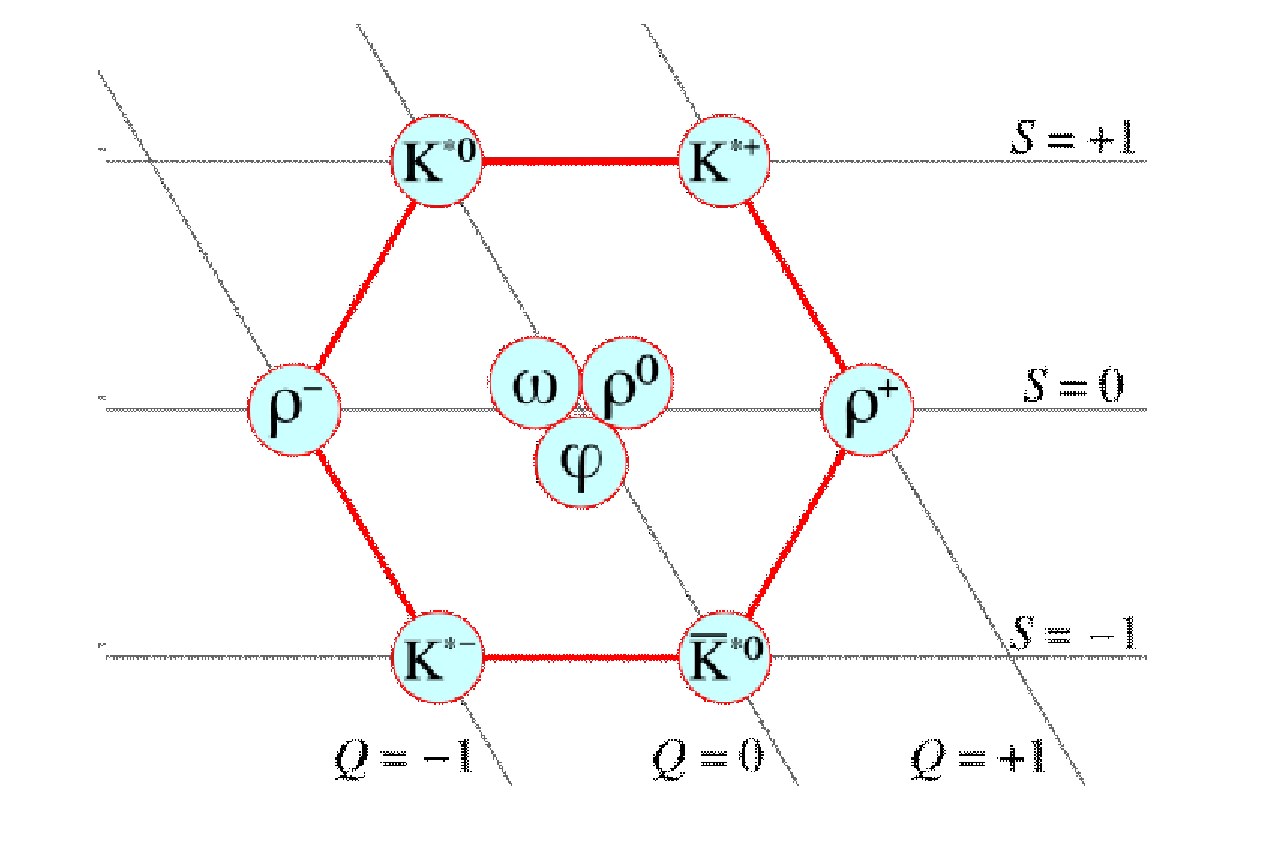
\includegraphics[width=8.5cm]{vector.eps}
  \caption{nonet of vector mesons}
  \label{fig:vector}
  \end{minipage}
\end{figure}
The different types are shown in Table \ref{tab:typemeson}. The nonet of the pseudoscalar mesons ($J^P=0^-$) and the nonet
of the vector mesons are shown in Figure \ref{fig:pseudoscalar} and Figure
\ref{fig:vector}. Here the charge increases towards the right and the
strangeness increases towards the upward direction. Note, that $\eta$ and $\eta'$ are not the exact octet and singlet
states, respectively. These are denoted by $\eta_0$ and $\eta_8$. The physical, measured particles
are mixings between the $\eta_0$ and $\eta_8$ states with an $\eta$-$\eta'$-mixing
angle $\theta_{mix} \approx - 20^\circ$ \cite{Holstein}. These states can be constructed from the flavor states
according to
\begin{equation}
\begin{pmatrix} \eta \\ \eta'  \end{pmatrix} =  \begin{pmatrix}  -\sin
  \theta_{{\rm mix}} & \cos \theta_{{\rm mix}}  \\ \cos \theta_{{\rm mix}} & \sin
  \theta_{{\rm mix}}   \end{pmatrix} \cdot \begin{pmatrix} \eta_0 \\ \eta_8  \end{pmatrix}.
\end{equation}

Since we want to study the decay of the pseudoscalar mesons $\pi^0, \eta$ and
$\eta'$, we first give some general informations of this particles and then
show their different decay modes.

\bigskip

The $\eta$ and $\eta'$ have a strange quark content:
\begin{eqnarray}
 \eta_8 &:& \frac{1}{\sqrt{6}}\left(u \bar u  + d \bar d  - 2 s \bar s \right),\\
 \eta_0 &:& \sqrt{\frac{2}{3}}\left(u \bar u  + d \bar d  +  s \bar s \right).
\end{eqnarray}
The masses of the mesons are $m_\eta = 547.853 \pm 0.024 \, {\rm MeV}$ and
$m_{\eta'}=(957.78 \pm 0.06) \, {\rm MeV} $. The decay modes and branching ratios are
given in Table \ref{tab:eta} and Table \ref{tab:eta'}.
\begin{table}[!htp]
\begin{center}
\renewcommand{\arraystretch}{1.08}
{\small
\begin{tabular}{l|c}												
Mode	& Branching ratio \\ \hline \hline	
$\eta \to 2\gamma$	 &   $ (39.30 \pm 0.20)  \cdot 10^{-2}$ \\
$\eta \to 3 \pi^0$  &  $ (32.56 \pm 0.23)  \cdot 10^{-2}$ \\
$\eta \to \pi^0 2\gamma$	 &  $(2.7 \pm 0.5)  \cdot 10^{-4}$\\
$\eta \to \pi^0 \pi^0 \gamma \gamma$  &  $<1.2 \cdot 10^{-3}$\\
$\eta \to 4 \gamma$  &  $<2.8 \cdot 10^{-4}$\\
$\eta \to$ invisible  &  $<6 \cdot 10^{-4}$\\
$\eta \to \pi^+ \pi^- \pi^0$  &  $ (22.73 \pm 0.28 ) \cdot 10^{-2}$\\
$\eta \to \pi^+\pi^- \gamma$ & $ (4.60 \pm 0.16)  \cdot 10^{-2}$\\
$\eta \to e^+ e^- \gamma$  &  $ (7.0 \pm 0.7)  \cdot 10^{-3}$\\
$\eta \to \mu^+\mu^- \gamma$  &  $ (3.1 \pm 0.4) \cdot 10^{-4}$\\
$\eta \to e^+ e^-$  &  $<2.7 \cdot 10^{-5}$ \\
$\eta \to \mu^+\mu^-$  &   $(5.8 \pm 0.8) \cdot 10^{-6}$\\
$\eta \to e^+ e^- e^+ e^-$  &  $<6.9 \cdot 10^{-5}$\\
$\eta \to \pi^+ \pi^- e^+ e^- $  &  $ (4.2- 1.3+ 1.5 ) \cdot 10^{-4}$\\
$\eta \to e^+ e^- \mu^+ \mu^- $  &  $<1.6 \cdot 10^{-4}$\\
$\eta \to \mu^+\mu^-\mu^+\mu^-$  &  $<3.6 \cdot 10^{-4}$\\
$\eta \to \mu^+\mu^-\pi^+ \pi^-$  &  $<3.6 \cdot 10^{-4}$\\
$\eta \to \pi^+ \pi^- 2\gamma$  &  $<2.0 \cdot 10^{-3}$\\
$\eta \to \pi^+ \pi^-\pi^0 \gamma$  &  $<5 \cdot 10^{-4}$ \\
$\eta \to \pi^0 \mu^+ \mu^- \gamma $  &  $<3 \cdot 10^{-6}$
\end{tabular}
  \caption{branching ratios of the $\eta$ decays \cite{Amsler}\label{tab:eta}}}
\end{center}
  
\end{table}

\newpage

\begin{table}[!htp]
\begin{center}
\renewcommand{\arraystretch}{1.08}
{\small
\begin{tabular}{l|c}												
Mode	& Branching ratio \\ \hline \hline
$\eta' \to \pi^+ \pi^- \eta$  &  $ (44.6 \pm 1.4) \cdot 10^{-2}$\\
$\eta' \to \rho_0 \gamma$ (including non-resonant $\pi^+ \pi^- \gamma$)  &  $(29.4 \pm
0.9) \cdot 10^{-2}$ \\
$\eta' \to \pi^0 \pi^0 \eta$  &  $ (20.7 \pm 1.2) \cdot 10^{-2}$ \\
$\eta' \to \omega \gamma$&  $ (3.02 \pm 0.31) \cdot 10^{-2}$ \\
$\eta' \to \gamma \gamma$  &  $(2.10 \pm 0.12) \cdot 10^{-2}$ \\
$\eta' \to 3 \pi^0$  &  $(1.61 \pm 0.23 ) \cdot 10^{-3}$\\
$\eta' \to \mu^+ \mu^-\gamma$  &  $( 1.03 \pm 0.26 ) \cdot 10^{-4}$\\
$\eta' \to \pi^+ \pi^- \mu^+ \mu^-$  &  $<2.3 \cdot 10^{-4}$\\
$\eta' \to \pi^+ \pi^- \pi^0$  &  $( 3.7- 1.0+ 1.1 ) \cdot 10^{-3}$\\
$\eta' \to \pi^0 \rho ^0$  &  $<4 \cdot 10^{-2}$\\
$\eta' \to 2(\pi^+ \pi^-)$  &  $<2.5 \cdot 10^{-4}$ \\
$\eta' \to \pi^+ \pi^- 2 \pi^0$  &  $<2.6 \cdot 10^{-3}$ \\
$\eta' \to 2(\pi^+\pi^-)$ neutrals  &  $<1 \cdot 10^{-2}$\\
$\eta' \to 2(\pi^+ \pi^-) \pi^0$  &  $<1.9 \cdot 10^{-3}$ \\
$\eta' \to 2(\pi^+\pi^-) 2\pi^0$  &  $<1 \cdot 10^{-2}$ \\
$\eta' \to 3(\pi^+\pi^-)$  &  $<5 \cdot 10^{-4}$\\
$\eta' \to \pi^+ \pi ^- e^+ e^-$  &  $( 2.5- 1.0+ 1.3 ) \cdot 10^{-3}$ \\
$\eta' \to e^+ e^- \gamma$  &  $<9 \cdot 10^{-4}$ \\
$\eta' \to \pi^0 \gamma \gamma$  &  $<8 \cdot 10^{-4}$ \\
$\eta' \to 4 \pi^0$  &  $<5 \cdot 10^{-4}$ \\
$\eta' \to e^+ e^- $  &  $<2.1 \cdot 10^{-7}$ \\
$\eta' \to invisible$  &  $<9 \cdot 10^{-4}$ 
\end{tabular}
  \caption{branching ratios of the $\eta'$ decays \cite{Amsler}\label{tab:eta'}}}
\end{center}
  
\end{table}

%%%%%%%%%%%%%%%%%%%%%%%%%%%%%%%%%%%%%%%%%%%%%%%%%%%%%%%%%%%%%%%%%%%%%%%%%%%%%%%%%%%%%%%%%%%%%%
\subsection{Symmetries and anomalies}
Transformations which do not change the physics of a system are symmetry
transformations. In classical physics this means that the
action and thereby the equation of motion are unchanged. In a quantum mechanical
formulation, a symmetry is given if the
Lagrangian is invariant under the respective
transformation. The relationship between symmetries and conversation laws is
expressed via the Noether theorem which says that for every continuous
transformation that leaves the action invariant there exists a time
independent classical charge $ Q $ and a corresponding conserved current
$\partial_\mu J^\mu = 0$.\\
There exist many different kinds of symmetries, which are all
realized by nature. Listed here are two examples:\\
\begin{itemize}
\item exact symmetry: examples for exact symmetries are the electromagnetic
  gauge $U(1)$ or the $SU(3)$ color symmetry of QCD;
\item anomalous symmetry: If a classical symmetry is broken in quantum physics it is
  called anomalous. It is not a true
  symmetry. An example is the axial $U(1)$ symmetry, which is the symmetry of interest here.
\end{itemize} 

The concept of anomalies was introduced by Adler, Bell and Jackiw \cite{Adler,Bell}. One will give a short
overview of the calculations given in Chapter 19 of
\cite{Peskin}.\\
In the massless Dirac
Lagrangian the left- and right- handed
fermions are decoupled and the Lagrangian is therefore invariant under the transformation of the fields\footnote[1]{The (standard) notation of the $\gamma$-matrices is according to \cite{Bjorken}. The parameter $\theta$ is real valued and $\varepsilon^{\mu\nu\alpha\beta}$ is the total antisymmetric tensor in 3+1 dimensions}:
\begin{equation}
\Psi \rightarrow \Psi' =
e^{- i \theta \gamma_5}\Psi
\label{trafoqed}
\end{equation}
The corresponding axial current
\begin{equation}
j_{5\mu} = \bar \Psi \gamma_\mu \gamma_5 \Psi   
\end{equation}
is classically conserved,
\begin{equation}
\partial^\mu j_{5\mu} = 0.
\label{classj}
\end{equation}

If $\Psi$ satisfies $(i\gamma_\mu\partial^\mu - m)\Psi = 0$, then
$$\partial^\mu j_{5\mu} = (\partial^\mu\bar{\Psi})\gamma_\mu\gamma_{5}\Psi - \bar{\Psi}\gamma_{5}\gamma_\mu\partial^\mu\Psi$$ $$= (im\bar{\Psi})\gamma_{5}\Psi - \bar{\Psi}\gamma_{5}(-im\Psi)$$ $$= 2im\bar{\Psi}\gamma_{5}\Psi = 0$$ when $m=0$.

This does not hold quantum mechanically when gauge fields are present. The axial vector
current is built from two fermion fields. Because
the product of two local operators can induce singularities, we separate their
locations $x$ and $y$, and take the limit $(y-x) \to 0$ in the
end. This is visualized in Figure \ref{fig:radcor}.\\
The lowest order contribution (without background gauge fields) results in zero, because we have to take the trace over three $\gamma$-matrices. The next
order contribution instead gives a nonvanishing result. Therefore the
divergence of the current has the following form,
\begin{equation}
\partial^\mu j_{5\mu} = - \frac{e^2}{16 \pi^2} \varepsilon^{\mu\nu\alpha\beta}
F_{\mu\nu}F_{\alpha\beta},
\label{ABJ}
\end{equation}
which is known as Adler-Bell-Jackiw anomaly \cite{Adler, Bell}. $F_{\mu\nu}$ is the electromagnetic field strength tensor, $F_{\mu\nu}=\partial_\mu A_\nu - \partial _\nu A_\mu$.
\begin{figure}[t]
\begin{center}
\includegraphics[width=15cm]{backgrgauge.eps}
  \caption{higher order radiative corrections of $\Psi(y) \bar\Psi (x)$}
\label{fig:radcor}
\end{center}
\end{figure}
\\
%%%%%%%%%%%%%%%%%%%%%%%%%%%%%%%%%%%%%%%%%%%%%%%%%%%%%%%%%%%%%%%%%%%%%%%%%%%%%%%%%%%%%%%%%%%%%%

The electromagnetic processes influenced by the Abelian axial anomaly \cite{Sanjin} are of considerable
theoretical interest. Among them are the transitions of the type $\gamma^*(q) \to P^+(p_1) P^0(p_2) P^-(p_3)$, where
$\gamma^*$ denotes a, generally, virtual ($q^2\neq 0$) photon $\gamma$, $P^\pm$ stands for a charged and $P^0$ for a neutral meson from the pseudoscalar nonet, 
up to the strangeness conservation (so that $P^\pm = \pi^\pm, K^\pm$ and 
$P^0 = \pi^0, \eta, \eta'$). 
These processes are supposedly influenced by the, colloquially called, ``box" axial anomaly, since on the microscopic level, the three pseudoscalar ($P$) mesons would couple to the photon through a four-vertex quark loop, like in Fig. \ref{figbox}. 

\begin{figure}[b!]
\begin{center}
\includegraphics[scale=0.8]{box3.eps}
\caption{A box diagrams for the process $\gamma^{*}\to \pi^+ \pi^0 \pi^-$.}
\label{figbox}
\end{center}
\end{figure}

In the chiral limit (where ${m_\pi=0}$) and the soft--point limit  (of vanishing 4-momenta of external particles, $p_j=0=q$), 
which is a reasonably realistic approximation at low energies at least for the lightest pseudoscalars -- the pions, the anomaly analysis predicts 
\cite{Adler} 
that the theoretical amplitude is exactly
\begin{equation}
A_{\gamma}^{3\pi}\equiv\lim_{m_{\pi}\to 0}F_\gamma^{3\pi}(p_1=0,p_2=0,p_3=0) = \frac{e \, N_c}{12\pi^2 \, f_\pi^3}  \, ,
\label{boxA}
\end{equation}
where $e$ is the proton charge, $N_c$ the number of quark colors, and the pion decay constant $f_\pi = (92.42 \pm 0.33)$ MeV, whereby 
$A_{\gamma}^{3\pi} = (9.72 \pm 0.09)\, {\rm GeV}^{-3}$.

On the other hand, the experimental knowledge of the processes that should be influenced by the ``box anomaly" is not at all satisfactory, being quite scant. For the $\gamma^*\to \pi^+\pi^0\pi^-$ processes, which should be best approximated by the anomaly prediction (\ref{boxA}) since it involves only the lightest pseudoscalars, there is only one
published 
experimental value for the amplitude at finite momenta $p_j$, i.e., the 
form factor $F_\gamma^{3\pi}(p_1,p_2,p_3)$. 
It was extracted from the cross-section measured \cite{Antipov} 
at Serpukhov in the transition $\pi^- \gamma^*\to \pi^0\pi^-$ through the 
Primakoff effect, so that its value
$F_\gamma^{3\pi}(expt) = 12.9 \pm 0.9 \pm 0.5 \, {\rm GeV}^{-3}$ 
really corresponds to the average value of 
the form factor over the momentum range covered by the experiment.
The $\pi^-$ scattering on electrons at CERN SPS yielded the total 
cross section \cite{Sanjin} consistent with the Serpukhov value. 
In the meantime, one still awaits the analysis of the measurements of this form factor performed at CEBAF \cite{Miskimen}.

Now, however, there are new hopes of more and better experimental knowledge of such processes, as new high-statistic data on the form factor for the $\pi^- \gamma^* \to \pi^- \pi^0$ transition are expected soon from the COMPASS Primakoff experiments at CERN \cite{Abbon}. 

Thus experiments (including radiative decays of $\eta$ and $\eta'$ from g11 and g12) may finally confirm the relation (\ref{ATAtheorem}) 
between the ``box anomaly" processes and the much 
better understood and measured ``triangle anomaly" processes, 
notably the $\pi^0(p)\to \gamma(k_{1})\gamma(k_{2})$ decay into two real photons,
$k_1^2=0=k_2^2$. 
Namely, the pertinent chiral-limit and soft-point amplitudes 
$A_{\pi}^{2\gamma}$ and $A_{\gamma}^{3\pi}$ are related 
\cite{Adler} as
\begin{equation} 
A_{\pi}^{2\gamma} \, = \, {e f_\pi^2} \, A_{\gamma}^{3\pi}.
\label{ATAtheorem}
\end{equation}


\paragraph{Wess-Zumino-Witten Lagrangian} 
The Wess-Zumino-Witten Lagrangian consists of terms like: 
\begin{equation}
 A = \frac{N_{c} e^2}{96 \pi^2 f_\pi^2} \pi^0 \varepsilon^{\mu\nu\alpha\beta} F_{\mu\nu} F_{\alpha\beta},
\end{equation}
 which is the part that describes the the triangle anormally in the decay $\pi^0 \to
\gamma\gamma$,
and a term
\begin{equation}
B=-\frac{1}{12}\frac{N_{c}}{\pi^2
  f_\pi^3}\epsilon^{\mu\nu\alpha\beta}A_\mu\partial_\nu \pi^+ \partial_\alpha
\pi^- \partial_\beta \pi^0,
\end{equation}
that describes the coupling of a photon to three pseudoscalar mesons ($\gamma\pi^{+}\pi^{}\pi^{-}$ - vertex)
and therefore the decays $\eta/\eta' \to \pi^+\pi^-\gamma$. \\
In summary the
Wess-Zumino-Witten Lagrangian already determines the triangle anomaly sector
via $A$ and the box anomaly sector via $B$.

\subsection{Radiative Decay Rate}
Radiative decays are known to be very sensitive tools to explore decay mechanisms. Especially, when studied together with two hadrons as decay products, they enable us to adjust the invariant mass of the two-hadron system via a variation of the photon energy without interference of strong three-body final state interactions.

For the transitions at hand, the spectral decay data are fitted with a function of the form
\begin{equation}
\dfrac{d\Gamma(\eta\rightarrow\pi^{+}\pi^{-}\gamma)}{ds_{\pi\pi}} = |AP(s_{\pi\pi})F_{V}(s_{\pi\pi})|^{2}\Gamma_{0}(s_{\pi\pi}),
\label{eqa}
\end{equation}
where the normalization parameter $A$ has the dimension of mass$^{-3}$, $s_{\pi\pi}$ is the invariant mass squared of $\pi^{+}\pi^{-}$ and where
\begin{equation}
\Gamma_{0}(s_{\pi\pi})=\frac{1}{3 \cdot 2^{11} \cdot \pi^{3} M_{\eta}^{3}}(M_{\eta}^{2} - s_{\pi\pi})^{3}s_{\pi\pi} \cdot \beta^{3}_{\pi}
\end{equation}
is the simplest gauge-invariant matrix element multiplied by the phase-space term $\beta_{\pi} = \sqrt{1-4M_{\pi}^{2}/s_{\pi\pi}}$ and $F_{V}(s_{\pi\pi})$ is the pion vector from factor, approximation in the energy range of interest by the polynomial $|F_{V}(s_{\pi\pi})|= 1+(2.12\pm 0.01)s_{\pi\pi}+(2.13\pm 0.01)s_{\pi\pi}^{2}+(13.80\pm 0.14)s_{\pi\pi}^{3}$.
The $P(s_{\pi\pi})$ function, a process-specific part, can be treated perturbatively in the frame of ChPT, for decay of light mesons. Taylor expansion around $s_{\pi\pi}=0$ gives
\begin{equation}
P(s_{\pi\pi}) = 1 + \alpha \cdot s_{\pi\pi} + O (s_{\pi\pi})
\label{eqb} 
\end{equation}

The parameters $\alpha$ allow insights into the physics underlying the decay process.

%%%%%%%%%%%%%%%%%%%%%%%%%%%%%%%%%%%%%%%%%%%%%%%%%%%%%%%%%%%%%%%%%%%%%%%%%%%%%%%%%%%%%%%%%%%%%%  

\section{Experimental Setup}

The data to be used in this analysis are from part of the g11a experiment, 
which was taken from May 17 to July 29, 2004, using the CEBAF Large 
Acceptance Spectrometer (CLAS) located in  Hall-B  at the Thomas 
Jefferson National Accelerator Facility (TJNAF). 
Real photons were produced by bremsstrahlung from a 4.0186 GeV 
electron beam incident on a 1 $\times$ 10$^{-4}$ radiation length gold foil.
The electron beam was delivered by the Continuous Electron Beam 
Accelerator Facility (CEBAF). 
The Hall-B Tagging System was used to determine the 
photon energies by measuring the energies of the recoil electrons 
using a dipole magnetic field and a scintillator hodoscope. 
The associated photon energies were then calculated by the difference 
between the incident electron energies and the recoil electron energies.\\ 
\indent A liquid hydrogen target was used in the g11a experiment.  The 
target was contained in a cylindrical Kapton chamber of 2 cm radius and 40 cm length.\\
\indent The CLAS apparatus was used to detect particles generated from the 
interaction of the incident photons with the target. 
The CLAS detector was able to track charged particles that have momenta 
larger than $\sim$200 MeV, and the detection area covered polar angles 
from 8$^{\circ}$ to 142$^{\circ}$ and 80\% of the azimuthal region.  
It was composed of several sub-systems, arranged with 
a six-fold azimuthal symmetry. 
A plastic scintillator Start Counter, placed just outside of the target, 
was used to measure the vertex time of particles in coincidence with 
the incoming photon.  
The superconducting coils of the CLAS detector generated a toroidal 
magnetic field that bent the path of outgoing charged particles. 
Those particles traveled through 3 regions of drift chambers that measured the curved paths to give the particle momenta. 
For the g11a experiment, the current in the superconducting coils was 
set at 1920 A, which gave a maximum magnetic field of $\sim$ 1.8 T. 
The time of flight (TOF) system was located beyond the outermost drift 
chambers at a radius of $\sim$4 m from the target and was used to measure the time and position of each charged 
particle that hit the TOF scintillators. 
The TOF information, along with the particle momentum, was used for 
the particle identification in the analysis.  
The time resolution of the TOF system was about 80 ps to 160 ps, 
depending on the length of the scintillators. \\
\indent The event trigger for the g11a experiment required that at least 
two tracks were detected in different sectors of CLAS. 
Once the event satisfied this condition, it was written to tape for 
future analysis. 

\section{Data Analysis}

As one of the largest photoproduction datasets at CLAS, the g11a experiment 
has $\sim$20 billion triggers.  
 
\subsection{Channels of Interest}

Because the $\eta$ and $\eta^{'}$ are unstable, they will quickly decay 
into the lighter $\pi$-mesons and/or $\gamma$(s) by the strong interaction. One is interested in the photoproduction channel(s):
\begin{equation}
\gamma p \to p \eta (\eta^{'})
\label{eq1}
\end{equation}
followed by
\begin{equation}  
 \eta \to \pi^{+} \pi^{-} \gamma       
\label{eq2}
\end{equation}
or
\begin{equation}  
\eta^{'} \to \pi^{+} \pi^{-} \gamma.
\label{eq3}
\end{equation}

The $\eta$  and  $\eta^{'}$ are reconstructed using the missing mass technique.

\subsection{Event Selection and Particle Identification}

Events were selected with three charged tracks in the final state identified as a proton, $\pi^{+}$ and $\pi^{-}$ in addition to a photon tagged by an electron in the tagger. These particles were selected according to particle id assigned by the CLAS Simple Event Builder (SEB) package. In order to identify the type of particle, the SEB package calculates the velocity $\beta_{meas}$ of the detected particle and compares it with the expected $\beta_{cal}$ corresponding to the measured momentum and the masses of different possible types of particles. The particle type is chosen based on the minimum difference between the measured $\beta_{meas}$ and $\beta_{cal}$ velocities. 

\subsection{Cuts}
\label{cuts}

The decay of a pseudoscalar meson to $\pi^{+} \pi^{-} \gamma$ requires identification of final state separation of single photon from $\pi^{0}$.

Several cuts were applied to the data to reduce the background and 
to remove events below threshold for the reaction of interest.
In general, the strategy is to use kinematic 
constraints to eliminate backgrounds while ensuring that the 
signal remains robust. The efficiency of various cuts would later on be 
tested with Monte Carlo simulations.

The kinematic constraints used so far are listed below:
\begin{itemize}
\item
Figure \ref{fig:ME} shows the missing mass of all detected particles with a cut on
missing energy $|ME-E_{\gamma}| < 0.05$ GeV. This plot shows a peak around zero, but it doesn?t yet secure rejection of $\pi^{0}$
in the event.
\begin{figure}[t!]
\begin{center}
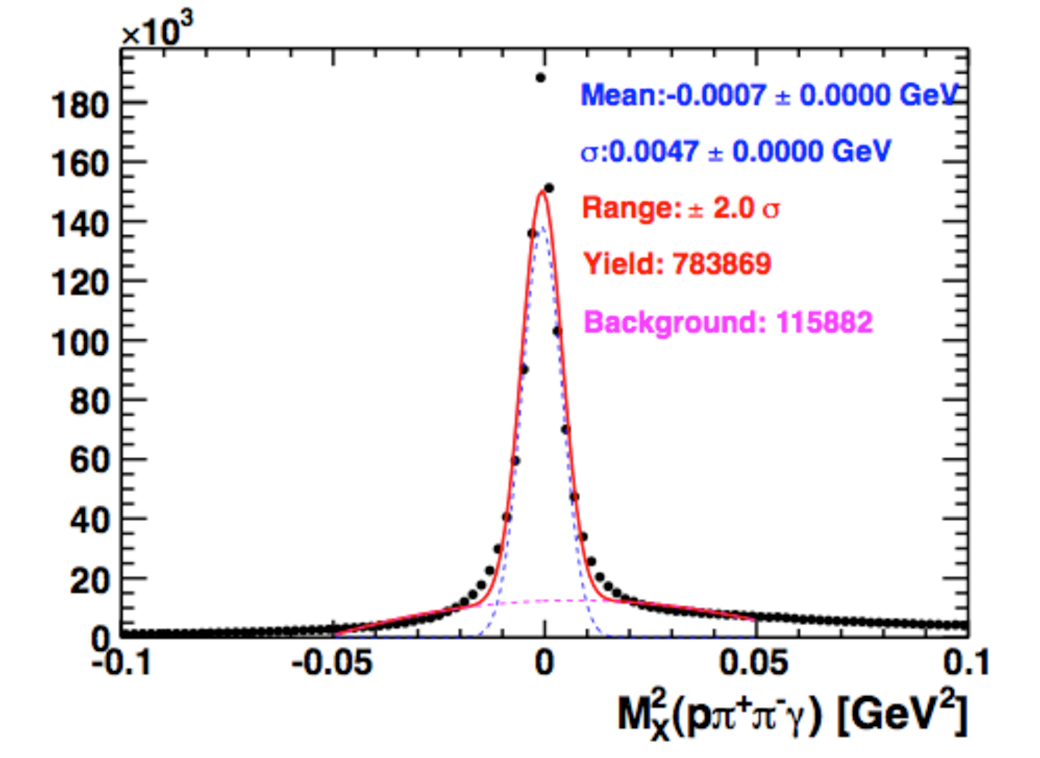
\includegraphics[width=12cm]{ME}
  \caption{Missing mass $M_{X}(p \pi^{+} \pi^{-} \gamma)$ of all detected final state particles.}
\label{fig:ME}
\end{center}
\end{figure}

\item
To ensure there is a $\pi^{0}$ amongst $p$, $\pi^{+}$ and $\pi^{-}$ in the final state, the square of the missing mass $M(p \pi^{+} \pi^{-})^{2}$ with additional cut $M(p \pi^{+} \pi^{-} \gamma)^{2} < 0.01$ GeV$^{2}$ for different ranges of missing mass $M_{X}(p)$ in the range of $\eta$, $\rho/\omega$ and $\eta^{'}$ is plotted (Figure \ref{fig:MM2}). One can clearly see the peaks of single $\gamma$ and $\pi^{0}$.  

\begin{figure}[h!]
\begin{center}
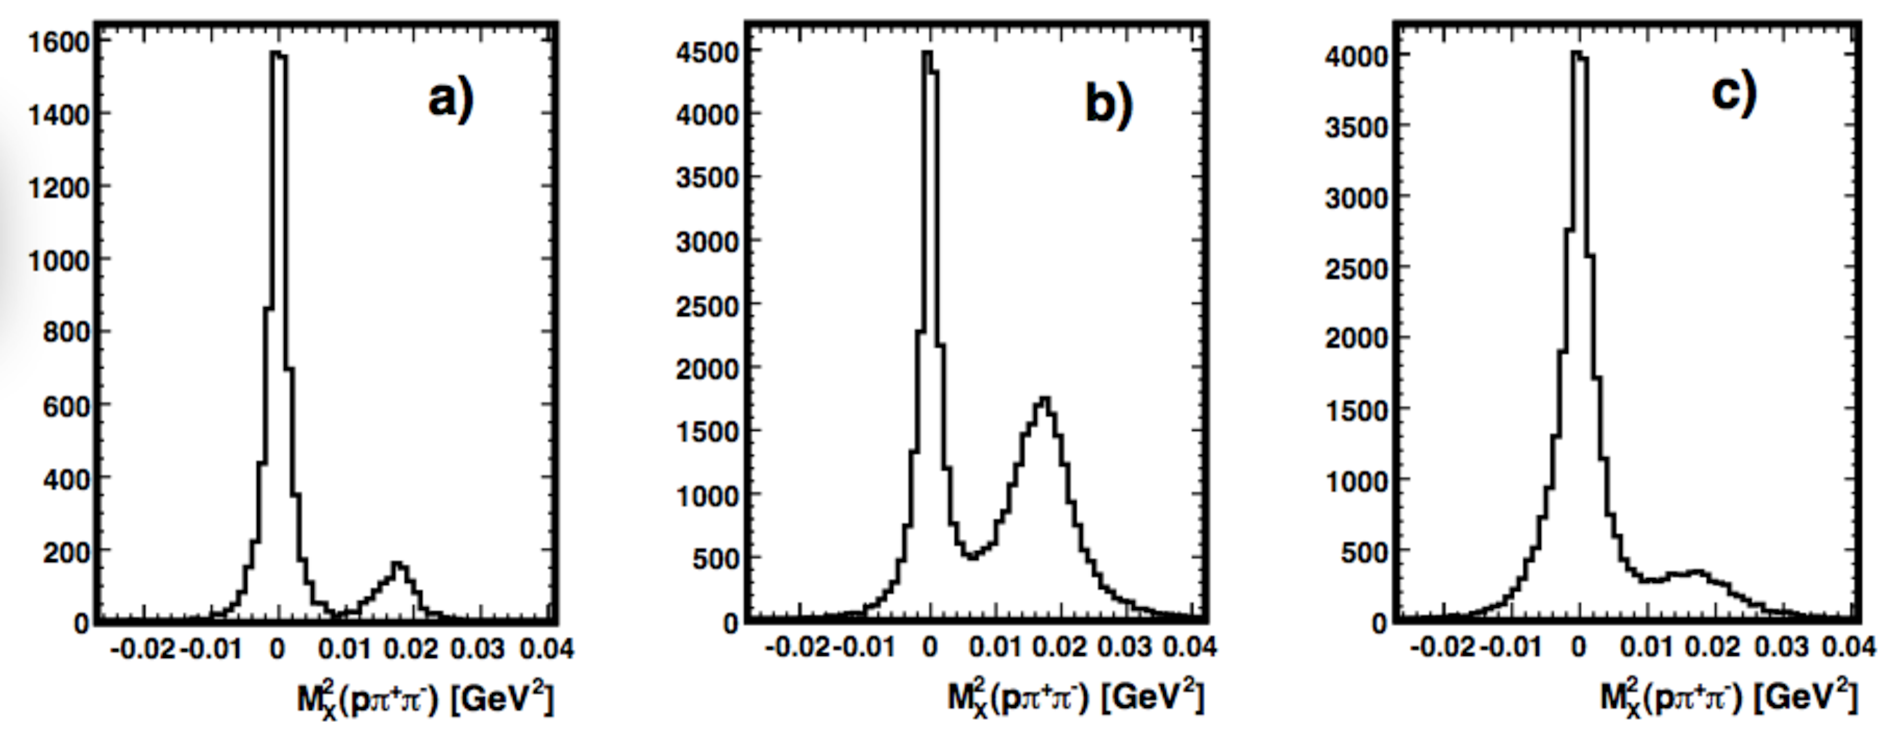
\includegraphics[width=15cm]{MM2}
  \caption{Distribution of events vs missing mass squared $M^{2}_{X}(p \pi^{+} \pi^{-} \gamma)$ for the range: a) $M_{X}(p) = 0.55 \pm 0.02$ GeV; b) $M_{X}(p) = 0.76 \pm 0.06$ GeV; c) $M_{X}(p) = 0.96 \pm 0.02$ GeV.}
\label{fig:MM2}
\end{center}
\end{figure}

\item
Reconstruction of all particles of interest with the best resolution was obtained by plotting the missing mass $M_{X}(p)$ with the cuts $M^{2}_{X}(p \pi^{+} \pi^{-} \gamma) < 0.01$ GeV$^{2}$ and $M^{2}_{X}(p \pi^{+} \pi^{-}) < 0.005$ GeV$^{2}$, Figure \ref{fig:MMP}.

\begin{figure}[h!]
\begin{center}
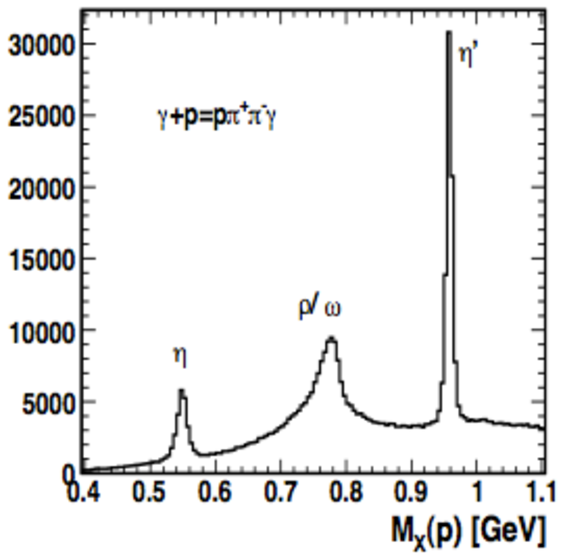
\includegraphics[width=8cm]{MMP}
  \caption{Distribution of missing mass of the proton in the exclusive reaction $\gamma p \rightarrow p \pi^{+} \pi^{-} \gamma$.}
\label{fig:MMP}
\end{center}
\end{figure}   

\end{itemize}

\section{CLAS preliminary versus world data}
\begin{figure}[h!]
\begin{center}
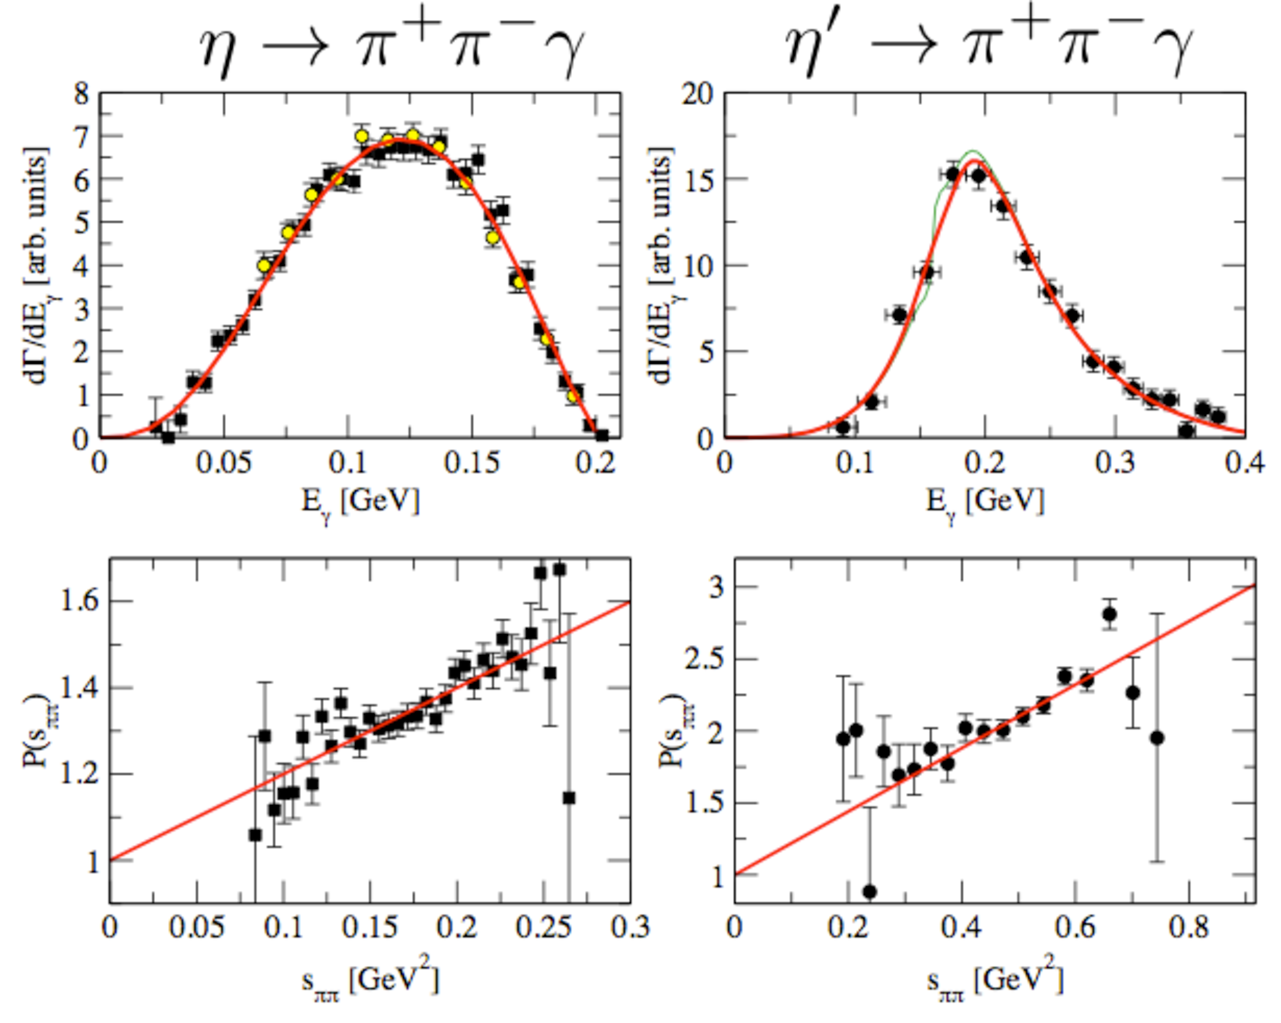
\includegraphics[width=12cm]{Egam_alpha}
  \caption{Top-left panel: distribution of $E_{\gamma}$ in cm frame of $\eta$. Top-right panel: same for $\eta^{'}$. Experimental data are from \cite{Adlarson,Abele}. Lower panel: Plot of $P(S_{\pi\pi})$, as extracted from the experimental data above.}
\label{fig:Egam_alpha}
\end{center}
\end{figure} 

\begin{figure}[h!]
\begin{center}
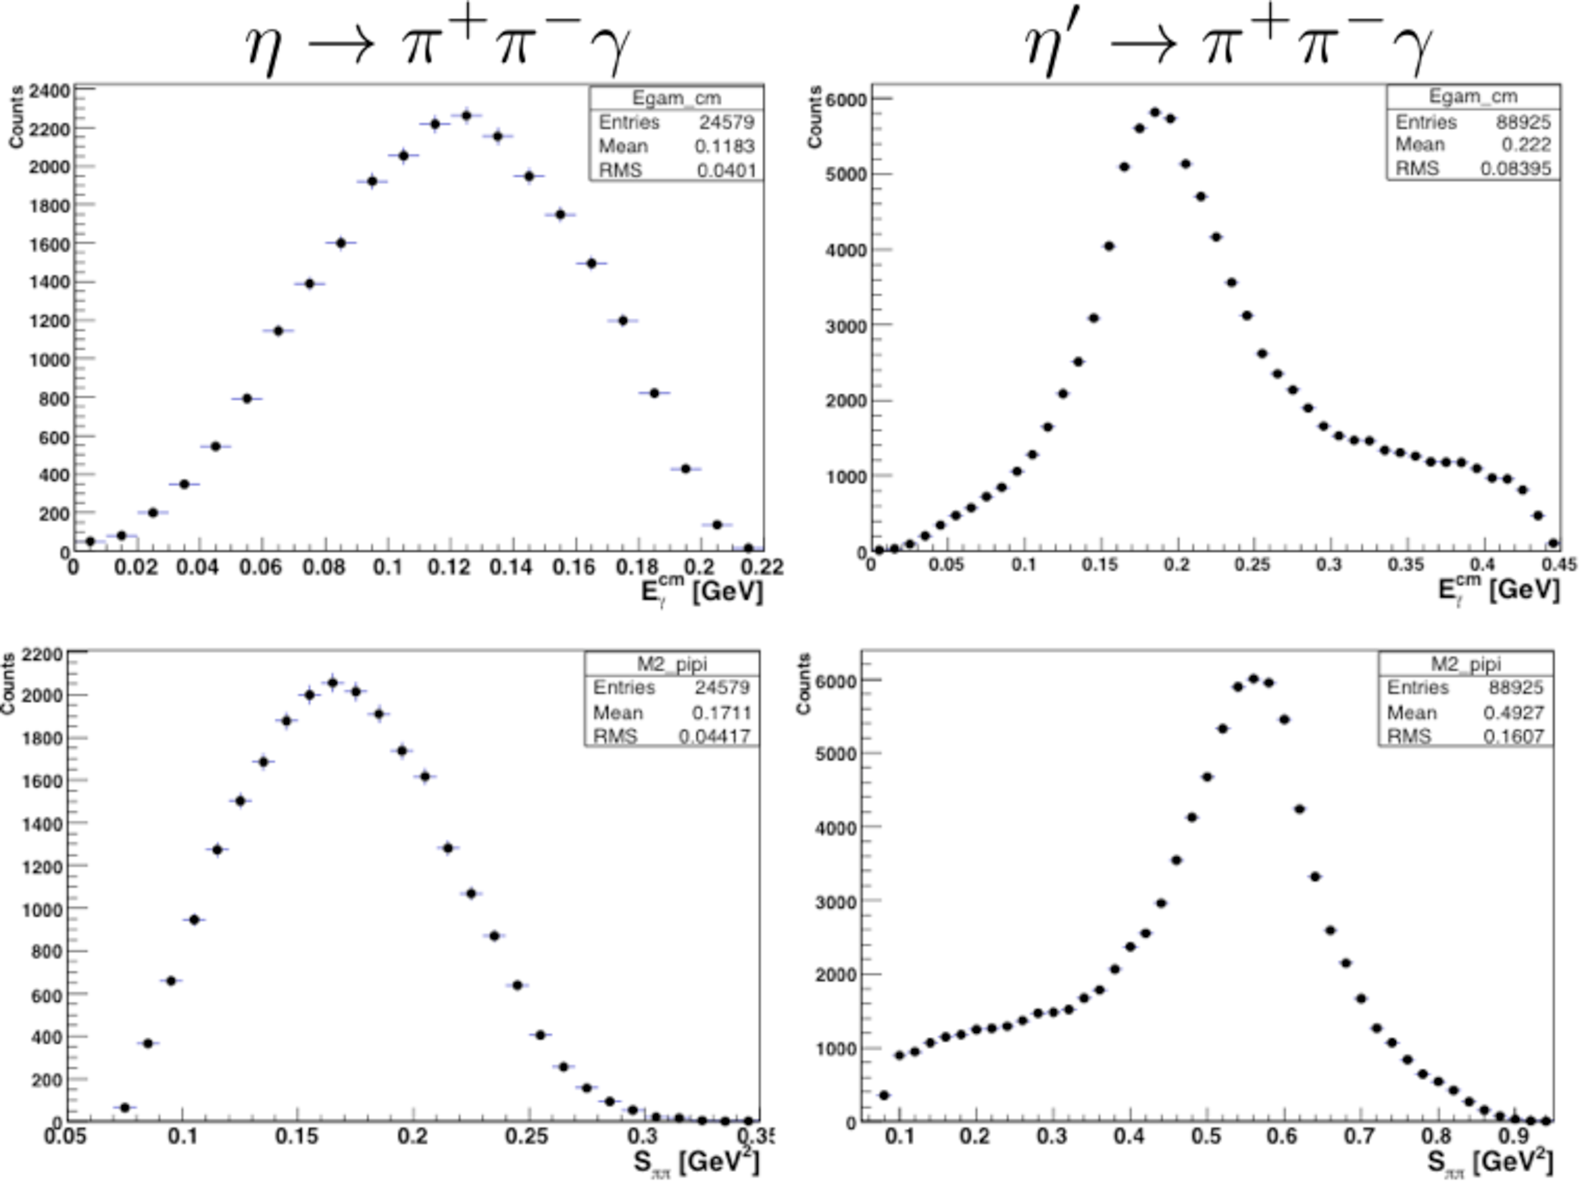
\includegraphics[width=12cm]{Egam_Spipi_data}
  \caption{Top-left panel: distribution of $E_{\gamma}$ in cm frame of $\eta$. Top-right panel: same for $\eta^{'}$. Lower-left panel: distribution of $E_{\gamma}$ in cm frame of $\eta$. Lower-right panel: same for $\eta^{'}$. Experimental data are from CLAS g11 data before acceptance and efficiency corrections.}
\label{fig:Egam_Spipi_data}
\end{center}
\end{figure} 

\begin{figure}[h!]
\begin{center}
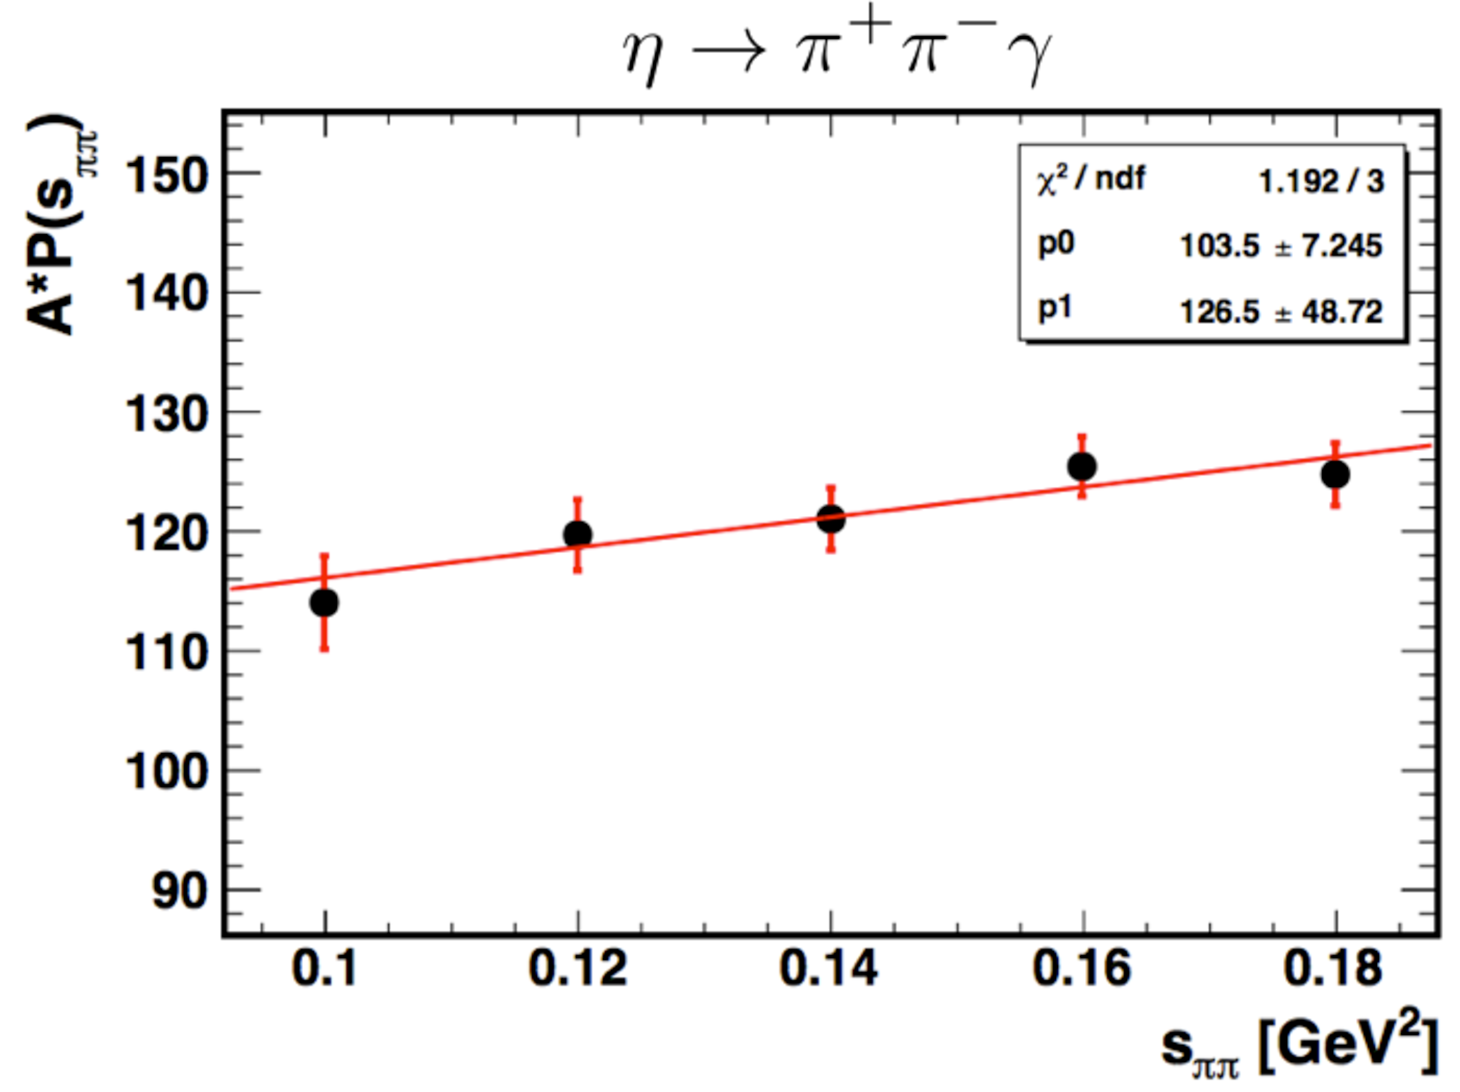
\includegraphics[width=12cm]{P_alpha}
  \caption{Very preliminary value for $\alpha = (1.22 \pm 0.47)$ GeV$^{-2}$ before acceptance and efficiency corrections.}
\label{fig:P_alpha}
\end{center}
\end{figure} 

Figure \ref{fig:MMP} represents the missing mass of the proton from g11 dataset for the exclusive reaction $\gamma p \rightarrow p \pi^{+} \pi^{-} \gamma$. In both the $\eta$ and $\eta^{'}$ peaks, the statistics is more than an order of magnitude higher than existing world data \cite{Moskov}. 

Figure \ref{fig:Egam_alpha} shows the center-of-mass photon energy distribution, $E^{cm}_{\gamma}$ for $\eta$ (top-left panel) and $\eta^{'}$ (top-right panel) from \cite{Adlarson, Abele}. The Lower panel shows plots of $P(S_{\pi\pi})$, Eqs.(12) and (14), as extracted from the experimental the mentioned experimental data.

The fits to the data points of the WASA-at-COSY collaboration \cite{Adlarson} for $\eta$ case and the CRYSTAL BARREL collaboration \cite{Abele} for the $\eta^{\prime}$ case give values:\\
$\alpha = (1.96 \pm 0.27 \pm 0.02)$ GeV$^{-2}$
and 
$\alpha^{\prime} = (1.80 \pm 0.49 \pm 0.04)$ GeV$^{-2}$
respectively.\\ 

Figure \ref{fig:Egam_Spipi_data} shows the center-of-mass photon energy distribution, $E^{cm}_{\gamma}$ for $\eta$ (top-left panel) and $\eta^{\prime}$ (top-right panel). The lower panels shows $s_{\pi\pi}$ for $\eta$ and $\eta^{\prime}$ from the CLAS g11 dataset before acceptance and efficiency corrections. $s_{\pi\pi}$ and $E^{cm}_{\gamma}$ are related by the expression:
\begin{equation}
s_{\pi\pi} = m^{2} - 2E_{\gamma}m
\end{equation}
where $m=m_{\eta}(m_{\eta^{\prime}})$.\\

Figure \ref{fig:P_alpha} shows the value of $\alpha$ extracted from five data points for the radiative decay of $\eta$. One is currently working on increasing the data points and extending the $s_{\pi\pi}$ range to around $0.25$ GeV$^{2}$. With a projection to reduce the statistical error to about that of the most recent result, $\alpha=(1.32\pm 0.08\pm 0.02)$ GeV$^{-2}$, from the KLOE Collaboration \cite{Kloe-2}. A similar procedure would be carried out for the $\eta^{\prime}$ decay, in CLAS. This measurement would provide the best statistical precision for $\alpha^{\prime}$ till date.  
  
\section{Expectations and Conclusion}
In conclusion, from the preliminary analyses done so far one can see that the CLAS data on the radiative decay of pseudoscalar mesons has high statistics compared to world data and can contribute significantly to essential topics of low energy QCD.

Ones immediate expectation is to use Monte Carlo simulations to carry on with acceptance and efficiency corrections so as to calculate the differential cross sections of the processes $\eta \rightarrow \pi^{+} \pi^{-} \gamma$ and $\eta^{\prime} \rightarrow \pi^{+} \pi^{-} \gamma$. Followed by making measurements of $E^{cm}_{\gamma}$ and $s_{\pi\pi}$ distributions in both processes and hence extract the model-independent $\alpha$ and $\alpha^{\prime}$ parameters.

\newpage

\begin{thebibliography}{99}

\bibitem{Samios}
N.~P.~Samios,
Phys. Rev. {\bf 121}, 275 (1961).

\bibitem{Beddal}
A.~Bedall,
Eur. Phys. J. {\bf C54}, 365 (2008).

\bibitem{Barker:2002}
A.~R.~Barker {\it et al.},
Phys. Rev. {\bf D67}, 033008 (2003).

\bibitem{Lih:2009}
C.~C.~Lih,
ARXIV:0912.2147

\bibitem{wasa}
M.~Berlowski {\it et al.},
Phys. Rev. {\bf D77}, 032004 (2008).

\bibitem{kloe}
KLOE,
F.~Ambrosino {\it et al.}, (2008),
ARXIV:0812.4830

%\cite{Abbon:2007pq}
\bibitem{Abbon}
  P.~Abbon {\it et al.}  [COMPASS Collaboration],
  %``The COMPASS Experiment at CERN,''
  Nucl.\ Instrum.\ Meth.\  A {\bf 577}, 455 (2007)
  [arXiv:hep-ex/0703049].
  %%CITATION = NUIMA,A577,455;%%

%\bibitem{Gao}
%D.~N.~Gao,
%Phys. Lett. {\bf A17}, 1583 (2002).

\bibitem{Wess}
J.~Wess and B.~Zumino,
Phys. Lett. {\bf B37}, 95 (1971).

\bibitem{Witten}
E.~Witten,
Nucl. Phys. {\bf B223}, 422 (1983).

\bibitem{Holstein}
B.~R. Holstein,
Phys. Scripta {\bf T99}, 55 (2002), hep-ph/0112150

\bibitem{Amsler}
Particle Data Group,
C.~Amsler {\it et al.},
Phys. Lett. {B667}, 1 (2008).

\bibitem{Adler}
S.~L.~Adler,
Phys. Rev. {\bf 177}, 2426 (1969).

\bibitem{Bell}
J.~S.~Bell {\it et al.}, {\bf A60}, 47 (1969).

\bibitem{Peskin}
M. E. Peskin, D. V. Schroeder, {\em An Introduction to Quantum Field Theory} (Addison-Wesley, USA, 1995).

\bibitem{Sanjin}
S. Beni\'{c} {it et al.}, 
arXiv: 1109.3140

\bibitem{Bjorken}
J. D. Bjorken and S. D. Drell, 
Bibliograph Inst./Mannheim 1967.

\bibitem{Antipov}
  Y.~M.~Antipov, V.~A.~Batarin, V.~A.~Bezzubov, N.~P.~Budanov, Y.~P.~Gorin, Y.~A.~Gornushkin, S.~P.~Denisov, S.~V.~Klimenko {\it et al.},
  %``Investigation Of Gamma ---> 3 Pi Chiral Anomaly During Pion Pair Production By Pions In The Nuclear Coulomb Field,''
  Phys.\ Rev.\  {\bf D36 } (1987)  21.
  
\bibitem{Miskimen} R. A. Miskimen, K. Wang, A. Yagneswaran (spokesmen),``Study of the Axial Anomaly using the $\gamma\pi^{+}\to\gamma\pi^{+}$ Reaction Near Threshold", letter of intent, CEBAF-experiment 94-015.  

\bibitem{Moskov}
M. J. Amaryan {\it et al.},
Photoproduction and Decay of Light Mesons in CLAS.

\bibitem{Adlarson}
P. Adlarson {\it et al.} (WASA@COSY Collaboration),
Phys. Lett. {\bf B707}, 243 (2012), 1107.5277.

\bibitem{Abele}
A. Abele {\it et al.} (Crystal Barrel Collaboration), 
Phys. Lett. {\bf B402}, 195 (1997). 

\bibitem{Stollenwerk}
F. Stollenwerk {\it et al.}  
arXiv: 1108.2419v3 (2011).

\bibitem{Kloe-2}
D. Babusci {\it et al.}  
arXiv: 1209.4611v2 (2012).

%\bibitem{Thimo}
%Thimo Petri,
%ARXIV:1010.2378

%\bibitem{Picciotto}
%C. Picciotto, Phys. Rev. D45, 1569 (1992).

\end{thebibliography}

\ed
